% =============================================================================
% DS 423 SA - Machine Learning with Large Datasets
% Group 11 - Face Mask Detection (Object Detection)
% Duy Tan University, Da Nang
%
% IMPORTANT: Compile this document with XeLaTeX (e.g. on Overleaf, set
% Menu -> Compiler -> XeLaTeX) so that the Times New Roman font is used
% correctly and Vietnamese characters (if added later) render properly.
% =============================================================================

\documentclass[12pt,a4paper]{article}

% ---------------------------------------------------------------- Fonts / XeLaTeX
\usepackage{fontspec}
\IfFontExistsTF{Times New Roman}{%
  \setmainfont{Times New Roman}
}{%
  \setmainfont{TeX Gyre Termes} % metric-compatible fallback if Times New Roman
                                 % is not installed on the compiling machine
}

% ---------------------------------------------------------------- Layout
\usepackage[a4paper,margin=1in]{geometry}
\usepackage{setspace}
\onehalfspacing

% ---------------------------------------------------------------- Graphics / tables / code
\usepackage{graphicx}
\usepackage{booktabs}
\usepackage{array}
\usepackage{float}
\usepackage{caption}
\usepackage{enumitem}
\usepackage{listings}
\usepackage{xcolor}
\usepackage{hyperref}
\hypersetup{
  colorlinks=true,
  linkcolor=black,
  urlcolor=blue,
  citecolor=black,
  pdftitle={Face Mask Detection - Group 11 - DS 423 SA},
  pdfauthor={Tran Van Truong, Nguyen Nhu Nguyen}
}

% ---------------------------------------------------------------- Header / Footer
\usepackage{fancyhdr}
\setlength{\headheight}{15pt}
\pagestyle{fancy}
\fancyhf{}
\fancyhead[L]{Duy Tan University, Da Nang}
\fancyhead[R]{DS 423 SA -- Group 11}
\fancyfoot[C]{\thepage}
\renewcommand{\headrulewidth}{0.4pt}

% ---------------------------------------------------------------- Code listing style
\definecolor{codebg}{RGB}{245,245,245}
\definecolor{codekeyword}{RGB}{0,0,180}
\definecolor{codecomment}{RGB}{95,130,95}
\definecolor{codestring}{RGB}{160,30,30}

\lstdefinestyle{pythonstyle}{
  backgroundcolor=\color{codebg},
  basicstyle=\ttfamily\footnotesize,
  keywordstyle=\color{codekeyword}\bfseries,
  commentstyle=\color{codecomment}\itshape,
  stringstyle=\color{codestring},
  numbers=left,
  numberstyle=\tiny\color{gray},
  stepnumber=1,
  numbersep=8pt,
  breaklines=true,
  breakatwhitespace=false,
  frame=single,
  rulecolor=\color{gray!40},
  showstringspaces=false,
  tabsize=4,
  language=Python
}
\lstset{style=pythonstyle}

\newcolumntype{L}[1]{>{\raggedright\arraybackslash}p{#1}}

\begin{document}

% =============================================================================
% TITLE PAGE
% =============================================================================
\begin{titlepage}
\centering
\vspace*{1cm}
{\Large \textbf{DUY TAN UNIVERSITY, DA NANG}}\\[0.3cm]
{\large Faculty of Information Technology}\\[2cm]

{\large DS 423 SA -- Machine Learning with Large Datasets}\\[1.5cm]

\rule{\linewidth}{0.5pt}\\[0.4cm]
{\Huge \textbf{Face Mask Detection}}\\[0.2cm]
{\Large An Object Detection Approach for Public-Health Mask Compliance Monitoring}\\[0.4cm]
\rule{\linewidth}{0.5pt}\\[2cm]

{\large \textbf{Group Number:} 11}\\[0.3cm]
{\large \textbf{Interest Area:} Object Detection}\\[1.5cm]

\begin{tabular}{ll}
\textbf{Member} & \textbf{Student ID} \\
Tran Van Truong (Data \& Analysis Lead) & 28211452515 \\
Nguyen Nhu Nguyen (Modeling \& Evaluation Lead) & 28211403542 \\
\end{tabular}

\vfill
{\large \today}
\end{titlepage}

\tableofcontents
\newpage

% =============================================================================
\section*{Abstract}
\addcontentsline{toc}{section}{Abstract}

Public-health monitoring systems increasingly rely on automated visual
inspection to verify mask compliance in crowded public spaces. This report
presents an object-detection pipeline that identifies human faces in images
and classifies each detected face as \textit{with mask}, \textit{without
mask}, or \textit{mask worn incorrectly}, together with the corresponding
bounding box. The pipeline covers data collection, cleaning, exploratory data
analysis, and feature engineering on the public Face Mask Detection dataset
(853 images, three classes), followed by transfer learning with a YOLOv8s
detector pretrained on COCO. The model was tuned and evaluated on a
consumer-grade laptop GPU (NVIDIA RTX 3050, 4GB VRAM), demonstrating that a
practical, resource-constrained deployment is feasible. Model performance is
reported using mean Average Precision (mAP) at multiple IoU thresholds,
Intersection-over-Union (IoU)-based matching, Precision, and Recall.

% =============================================================================
\section{Introduction and Problem Statement}

Manual verification of face-mask compliance in public spaces (transport
hubs, hospitals, shopping centers) is labor-intensive and does not scale to
the volume of people passing through such spaces every day. An automated
computer-vision system that can process a camera feed and flag individuals
who are not wearing a mask correctly would materially reduce the workload of
public-health staff and provide continuous, objective monitoring.

This project frames mask-compliance checking as an \textbf{object detection}
problem rather than a simple image-classification problem: a real image may
contain zero, one, or several faces, each of which must be independently
\textit{located} (bounding box) and \textit{classified} into one of three
categories:

\begin{itemize}[noitemsep]
    \item \texttt{with\_mask} -- the person is wearing a mask correctly.
    \item \texttt{without\_mask} -- the person is not wearing a mask.
    \item \texttt{mask\_weared\_incorrect} -- a mask is present but worn
          incorrectly (e.g., not covering the nose).
\end{itemize}

The goal of this project is to build, train, and evaluate an object
detector that solves this task accurately enough to be useful in practice,
while remaining trainable on a single consumer laptop GPU.

% =============================================================================
\section{Dataset}

\subsection{Source}
The project uses the publicly available \textbf{Face Mask Detection}
dataset (andrewmvd, 2020) hosted on Kaggle:
\url{https://www.kaggle.com/datasets/andrewmvd/face-mask-detection}.

\subsection{Description}
The dataset contains \textbf{853 images} annotated in Pascal-VOC XML format,
with a total of approximately \textbf{4,072 bounding boxes} across three
classes. Each XML annotation file specifies the image dimensions and, for
every face in the image, a class label and a bounding box
(\texttt{xmin}, \texttt{ymin}, \texttt{xmax}, \texttt{ymax}).

\subsection{Class Distribution}
Exploratory analysis (Section~\ref{sec:methodology}) shows a class
imbalance typical of real-world safety datasets: the majority of annotated
faces belong to the \texttt{with\_mask} class, while
\texttt{mask\_weared\_incorrect} is a minority class. This imbalance was
taken into account when splitting the data (stratified train/validation
split) and when interpreting per-class Precision/Recall results.

\begin{figure}[H]
    \centering
    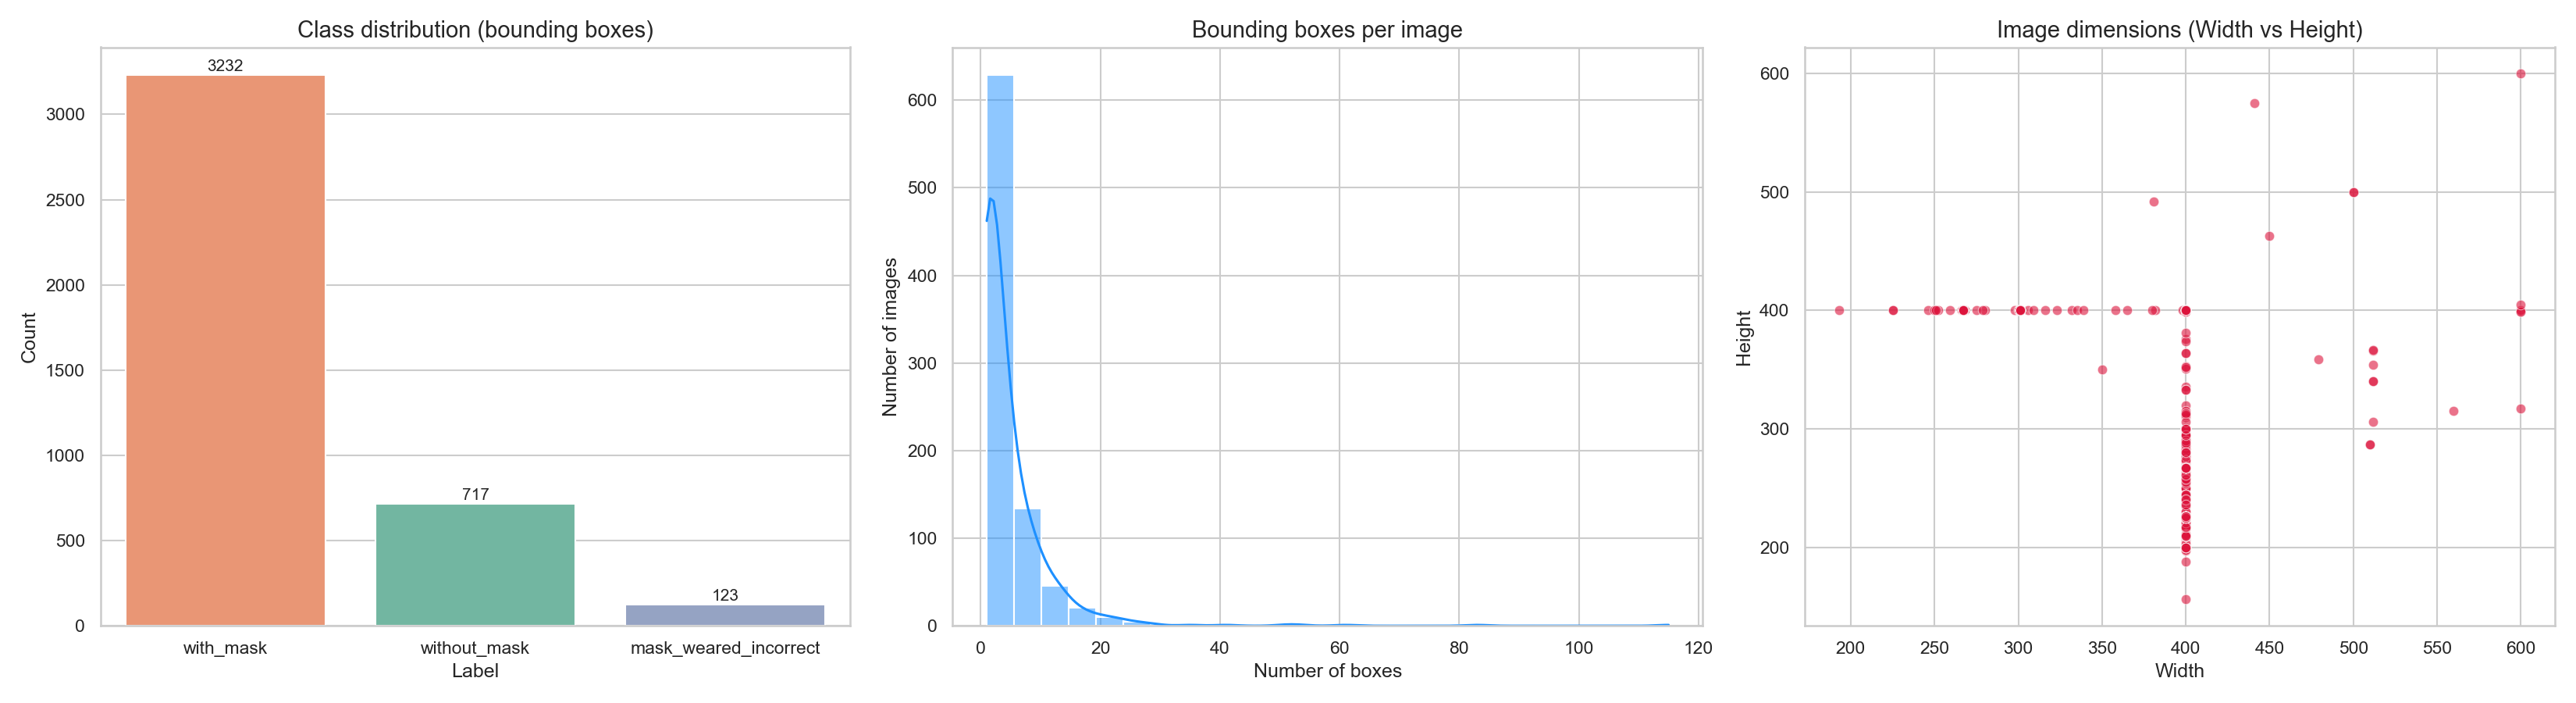
\includegraphics[width=0.95\linewidth]{report/figures/eda_overview.png}
    \caption{Exploratory Data Analysis: class distribution, number of
    bounding boxes per image, and image-size distribution.}
    \label{fig:eda}
\end{figure}

\subsection{Data Quality Issues Found and Corrected}
During data cleaning, a small number of bounding boxes were found to extend
one or more pixels beyond the image boundary (e.g., \texttt{xmax} slightly
larger than the recorded image width), most likely due to minor
inconsistencies between the XML metadata and the actual decoded image size.
Rather than discarding these boxes outright, they were \textbf{clamped to
the true image boundary} (as measured from the actual decoded image, not
just the XML metadata) and only dropped if they became degenerate
(zero or negative width/height) after clamping. This preserved more of the
already-limited training data while eliminating a bug that would otherwise
cause the annotation pipeline to raise coordinate-range errors during
training.

% =============================================================================
\section{Methodology}
\label{sec:methodology}

\subsection{Pipeline Overview}
The full pipeline is organized into ten parts inside a single Jupyter
notebook (\texttt{group11\_facemask.ipynb}), split according to each
member's assigned role:

\begin{enumerate}[noitemsep]
    \item Data collection and loading (parsing Pascal-VOC XML annotations).
    \item Data cleaning and preprocessing (missing values, out-of-bounds
          boxes, label encoding, verifying image files exist).
    \item Exploratory Data Analysis (class balance, boxes-per-image,
          image-size distribution, annotated sample images).
    \item Feature engineering (box width/height/area, aspect ratio,
          area ratio relative to image size).
    \item Stratified train/validation split (80/20).
    \item Model selection and building (dataset conversion to YOLO format;
          YOLOv8s initialization from COCO-pretrained weights).
    \item Training setup, hyperparameter tuning, and full training run.
    \item Evaluation (mAP, IoU-based Precision/Recall).
    \item Prediction visualization on validation samples.
    \item Saving the final model and a results summary table.
\end{enumerate}

\subsection{Model Selection}
\textbf{YOLOv8s} (Ultralytics) was selected as the detection model for the
following reasons:

\begin{itemize}[noitemsep]
    \item As a single-stage detector, YOLOv8 offers substantially faster
          training and inference than two-stage detectors such as Faster
          R-CNN, while still achieving competitive accuracy -- an important
          property for a system intended to eventually run on
          continuous video/camera streams.
    \item The "small" (\texttt{s}) variant balances accuracy and
          computational cost, fitting comfortably within the 4GB VRAM
          budget of the training GPU (NVIDIA RTX 3050 Laptop), unlike the
          larger \texttt{m}/\texttt{l}/\texttt{x} variants.
    \item Ultralytics YOLOv8 ships with COCO-pretrained weights, enabling
          transfer learning, which is essential given the relatively small
          size of the Face Mask Detection dataset (853 images).
    \item The \texttt{ultralytics} library provides built-in data
          augmentation, automatic mixed-precision (AMP) training, and
          native computation of mAP/Precision/Recall, reducing the amount
          of custom training code needed and the surface area for bugs.
\end{itemize}

\subsection{Data Conversion}
Because YOLO expects images and label files in its own format, the cleaned
annotations were converted from Pascal-VOC XML to YOLO text format: each
line \texttt{<class\_id> <x\_center> <y\_center> <width> <height>}, with all
four coordinates normalized to $[0,1]$ relative to the image size, and
\texttt{class\_id} converted from the 1-indexed label used earlier
(\texttt{with\_mask=1}, \texttt{without\_mask=2},
\texttt{mask\_weared\_incorrect=3}) to YOLO's required 0-indexed scheme.

\subsection{Training Configuration}
\begin{table}[H]
\centering
\caption{Training configuration used for the final YOLOv8s model.}
\label{tab:train-config}
\begin{tabular}{@{}ll@{}}
\toprule
\textbf{Setting} & \textbf{Value} \\
\midrule
Base weights & \texttt{yolov8s.pt} (COCO-pretrained) \\
Image size & $416 \times 416$ \\
Batch size & 8 \\
Epochs & 60 (early stopping, patience = 15) \\
Optimizer & Ultralytics \texttt{auto} optimizer \\
Initial learning rate (\texttt{lr0}) & 0.005 (selected via search) \\
Mixed precision (AMP) & Enabled \\
DataLoader workers & 0 (avoids multiprocessing issues on Windows) \\
Hardware & NVIDIA GeForce RTX 3050 Laptop GPU (4GB VRAM) \\
\bottomrule
\end{tabular}
\end{table}

\subsection{Hyperparameter Tuning}
A small hyperparameter search was performed over the initial learning rate
(\texttt{lr0} $\in \{0.01, 0.005, 0.001\}$), training each candidate for a
short number of epochs and comparing validation mAP@0.50. The best-performing
learning rate, \texttt{0.005},
was then used for the full 60-epoch training run. This search was
intentionally kept small in scope, given the time and compute constraints of
training on a single personal laptop.

% =============================================================================
\section{Implementation}

This section highlights the key parts of the implementation. The full,
runnable, and commented source code is provided in
\texttt{group11\_facemask.ipynb}.

\subsection{Converting Annotations to YOLO Format}
\begin{lstlisting}
def convert_split_to_yolo(data_list, images_out_dir, labels_out_dir):
    """Copy images and generate YOLO-format .txt annotation files
    for one split (train/val)."""
    n_boxes = 0
    for item in data_list:
        filename = item['filename']
        shutil.copyfile(item['image_path'],
                         os.path.join(images_out_dir, filename))

        img_w, img_h = item['width'], item['height']
        lines = []
        for (x1, y1, x2, y2), label_id in zip(item['boxes'], item['labels']):
            class_id = int(label_id) - 1  # YOLO expects 0-based ids
            x_center = min(max(((x1 + x2) / 2.0) / img_w, 0.0), 1.0)
            y_center = min(max(((y1 + y2) / 2.0) / img_h, 0.0), 1.0)
            box_w = min(max((x2 - x1) / img_w, 0.0), 1.0)
            box_h = min(max((y2 - y1) / img_h, 0.0), 1.0)
            lines.append(f"{class_id} {x_center:.6f} {y_center:.6f} "
                         f"{box_w:.6f} {box_h:.6f}")
            n_boxes += 1

        label_path = os.path.join(
            labels_out_dir, os.path.splitext(filename)[0] + ".txt")
        with open(label_path, "w") as f:
            f.write("\n".join(lines))
    return n_boxes
\end{lstlisting}

\subsection{Model Initialization and Training}
\begin{lstlisting}
from ultralytics import YOLO

model = YOLO("yolov8s.pt")   # COCO-pretrained weights

train_run = model.train(
    data=DATA_YAML_PATH,
    imgsz=416,
    batch=8,
    workers=0,               # avoid DataLoader issues on Windows
    device=device_str,       # '0' for GPU, 'cpu' otherwise
    seed=SEED,
    amp=True,                # mixed precision -> lower VRAM usage
    epochs=60,
    lr0=0.005,               # chosen via the hyperparameter search
    patience=15,             # early stopping
    project=OUTPUT_DIR,
    name="yolov8s_facemask_final",
    plots=True,
)
\end{lstlisting}

\subsection{Evaluation}
\begin{lstlisting}
map_results = model.val(
    data=DATA_YAML_PATH, imgsz=416, batch=8,
    device=device_str, workers=0, split="val"
)

print(f"mAP@[0.5:0.95] : {map_results.box.map:.4f}")
print(f"mAP@0.50       : {map_results.box.map50:.4f}")
print(f"mAP@0.75       : {map_results.box.map75:.4f}")
print(f"Precision (mp) : {map_results.box.mp:.4f}")
print(f"Recall (mr)    : {map_results.box.mr:.4f}")
\end{lstlisting}

In addition to the metrics computed natively by Ultralytics, a manual
IoU-based matching routine (using \texttt{torchvision.ops.box\_iou}) was
implemented to compute per-class Precision and Recall at a fixed IoU
threshold of 0.5, giving an explicit, independently verifiable view of the
IoU metric required by the assignment, separate from the internally
IoU-averaged mAP score.

% =============================================================================
\section{Results and Evaluation}

\subsection{Training Curves}
Figure~\ref{fig:loss} shows the training and validation loss (box-regression
loss and classification loss) across epochs.

\begin{figure}[H]
    \centering
    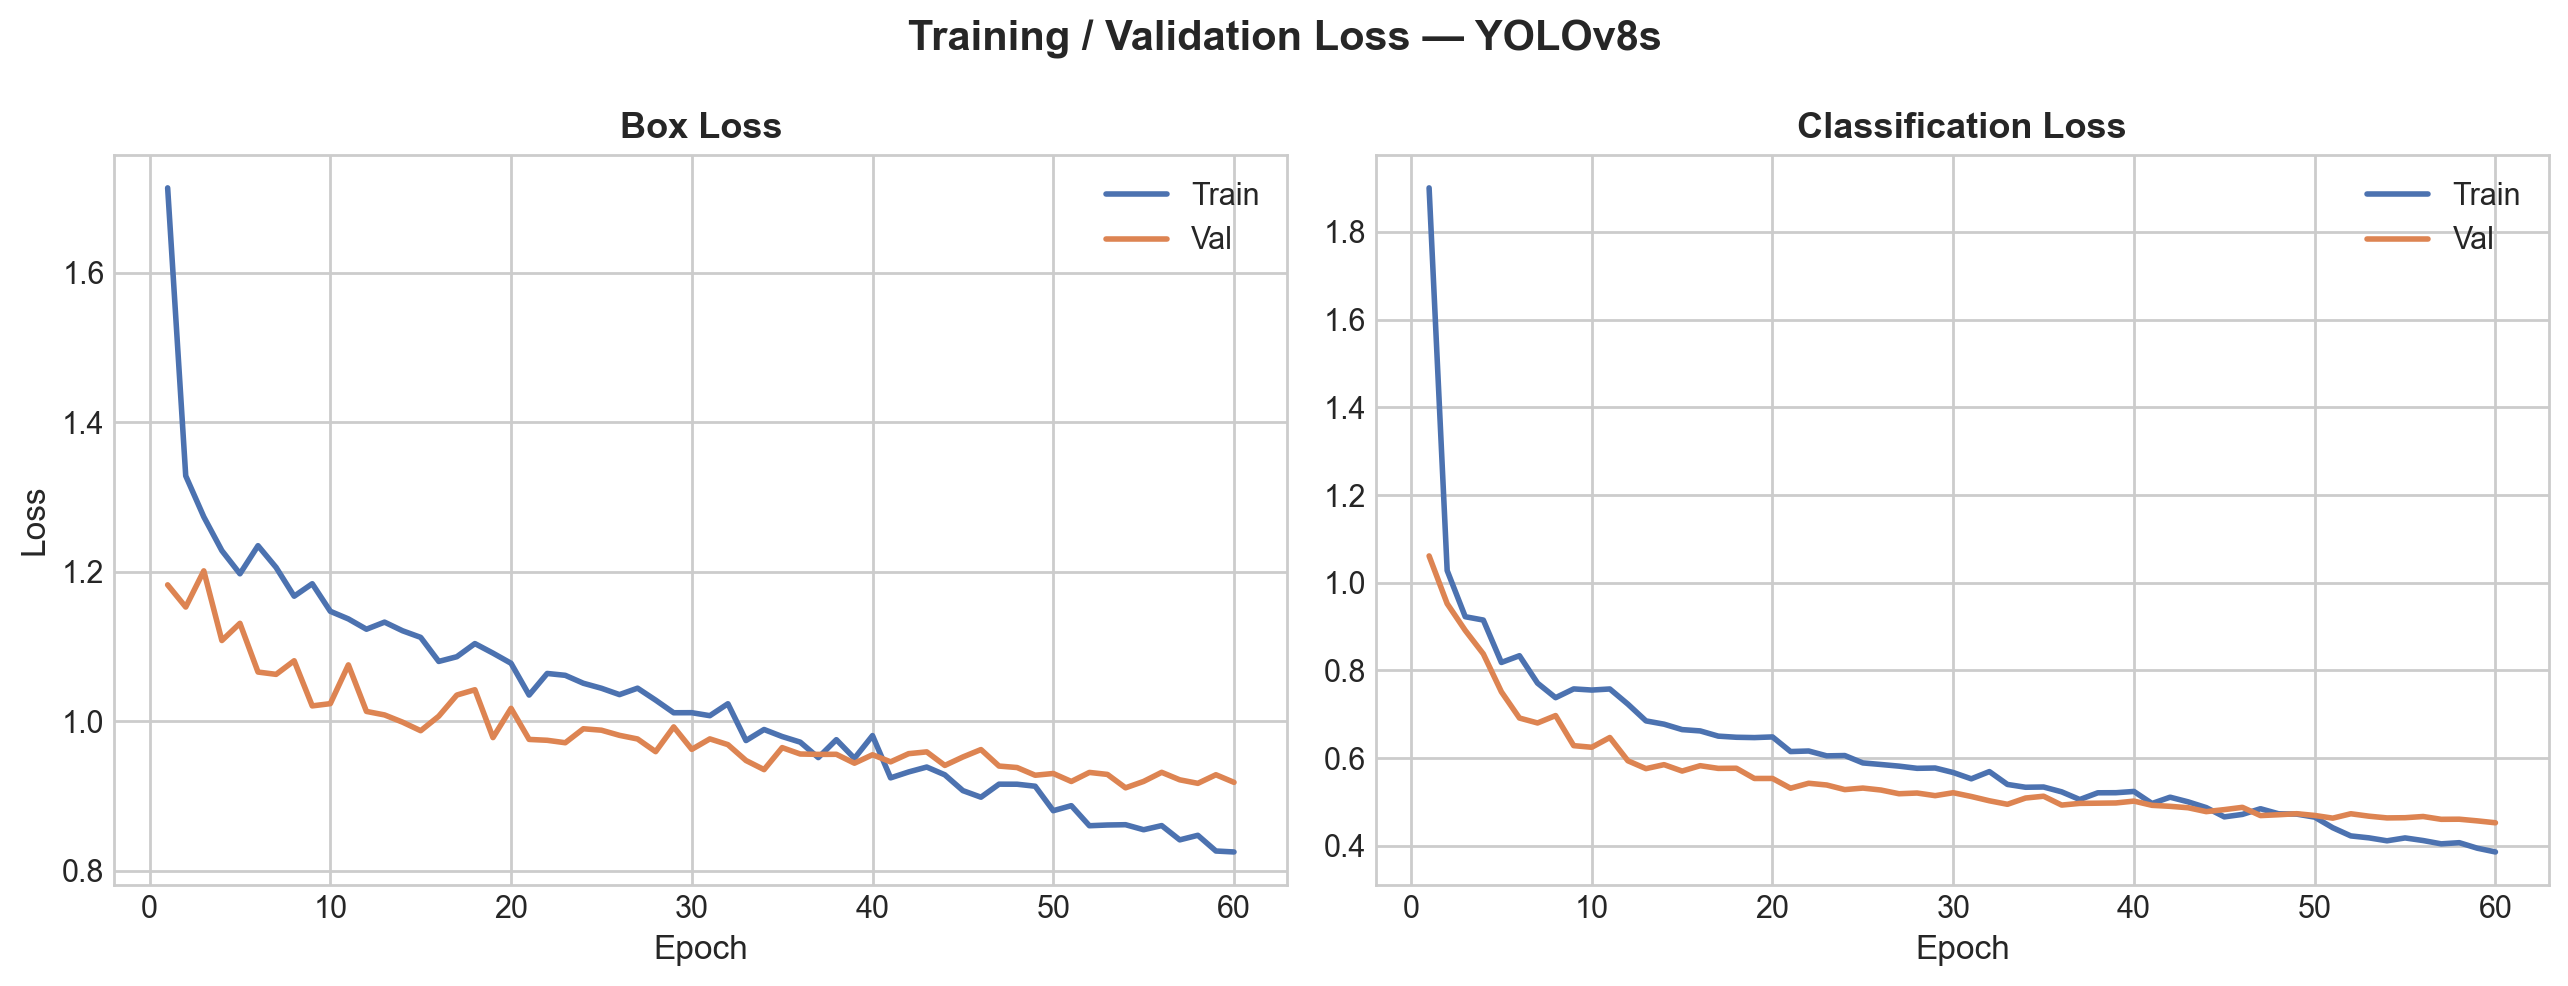
\includegraphics[width=0.95\linewidth]{report/figures/loss_curve.png}
    \caption{Training / validation loss curves for YOLOv8s.}
    \label{fig:loss}
\end{figure}

\subsection{Overall Metrics}
\begin{table}[H]
\centering
\caption{Overall detection performance on the validation split.}
\label{tab:overall-results}
\begin{tabular}{@{}lc@{}}
\toprule
\textbf{Metric} & \textbf{Value} \\
\midrule
mAP@[0.5:0.95] & 0.5723 \\
mAP@0.50       & 0.8186 \\
mAP@0.75       & 0.6795 \\
Precision (mean, IoU $\geq$ 0.5) & 0.9293 \\
Recall (mean, IoU $\geq$ 0.5)    & 0.7432 \\
\bottomrule
\end{tabular}
\end{table}

\subsection{Per-Class Metrics}
Figure~\ref{fig:perclass} shows Average Precision, Precision, and Recall
broken down by class, computed at an IoU threshold of 0.5.

\begin{figure}[H]
    \centering
    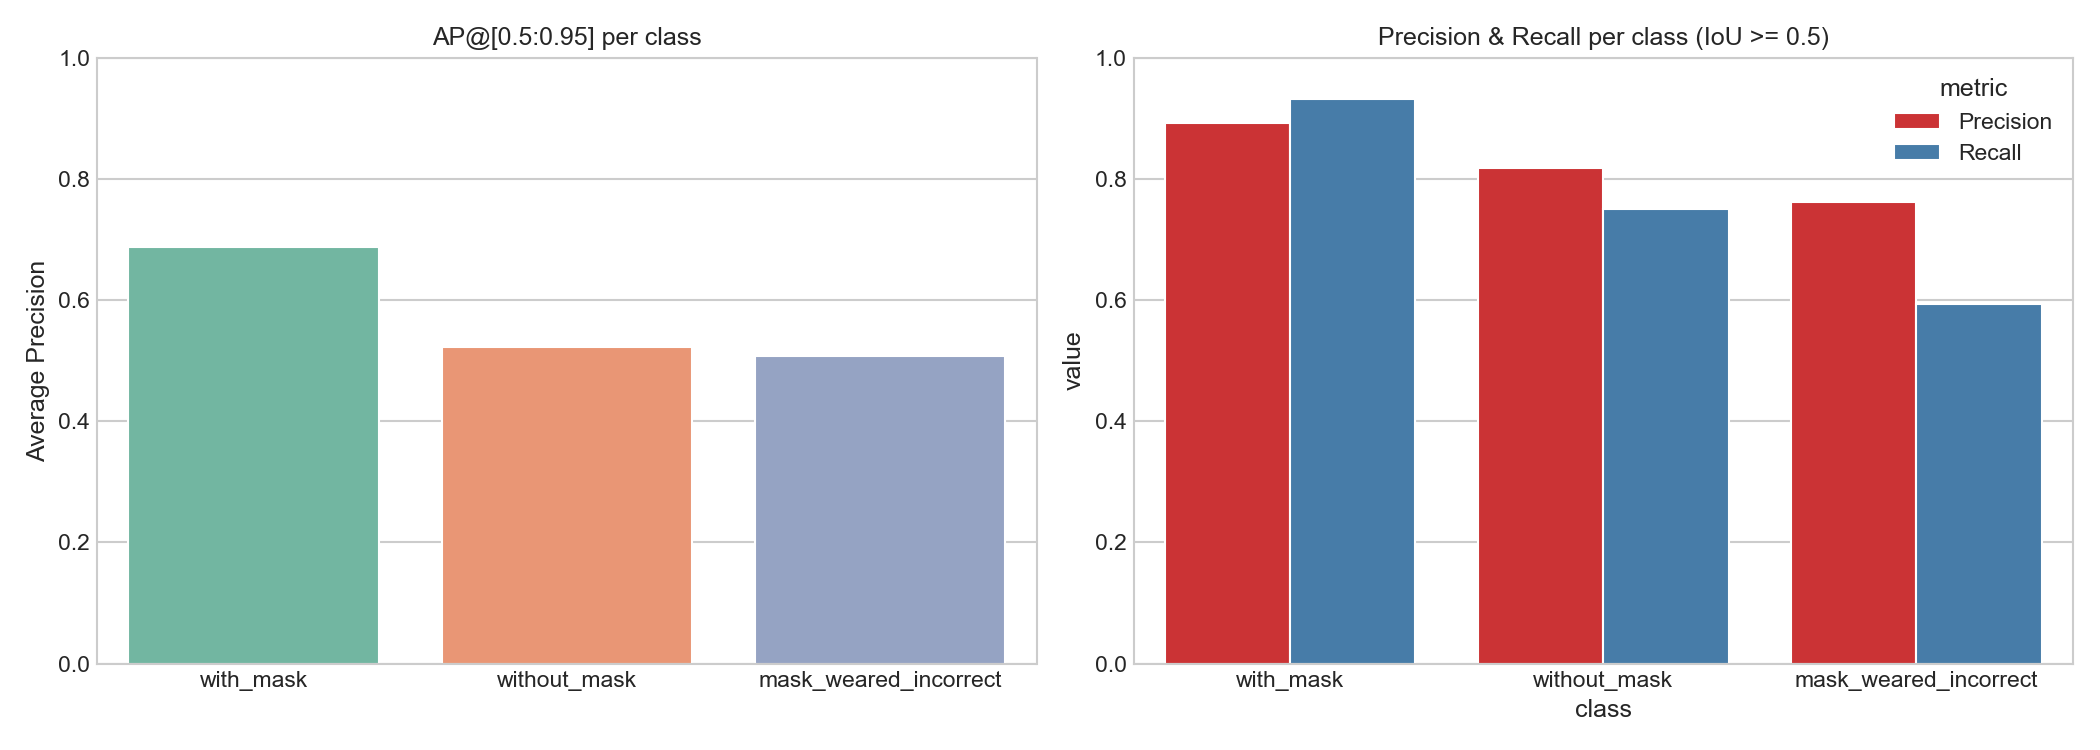
\includegraphics[width=0.95\linewidth]{report/figures/ap_precision_recall_per_class.png}
    \caption{Per-class AP@[0.5:0.95] and Precision/Recall at IoU $\geq$ 0.5.}
    \label{fig:perclass}
\end{figure}

The per-class chart shows that \texttt{with\_mask} obtains the strongest AP and recall, while \texttt{mask\_weared\_incorrect} has the lowest AP and recall among the three classes. This is consistent with the dataset imbalance discussed in Section 3.3: the minority incorrect-mask class provides fewer visual examples, making it harder for the detector to learn robust boundary and class cues.

\subsection{Qualitative Results}
Figure~\ref{fig:samples} shows example predictions on validation images,
overlaid with predicted bounding boxes, class labels, and confidence scores.

\begin{figure}[H]
    \centering
    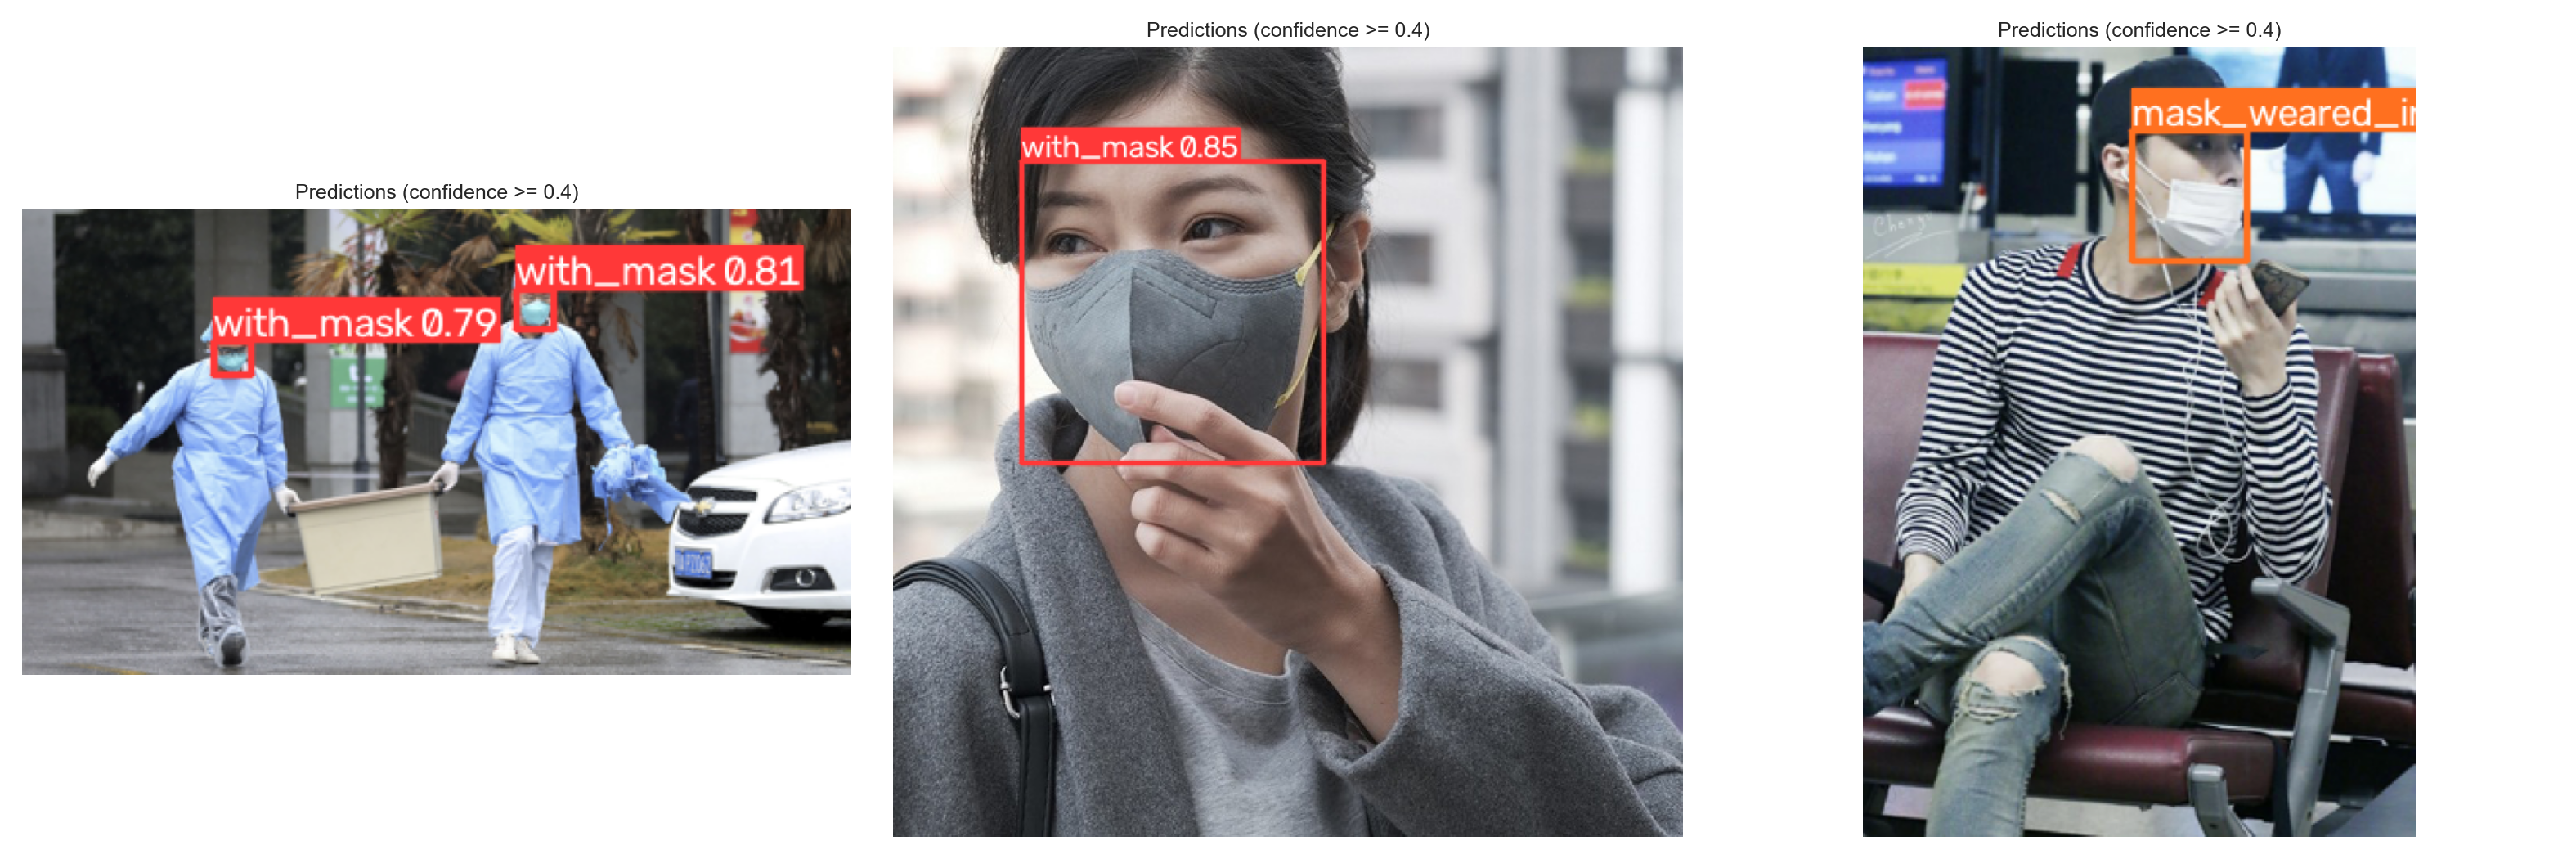
\includegraphics[width=0.95\linewidth]{report/figures/sample_predictions.png}
    \caption{Sample model predictions on validation images.}
    \label{fig:samples}
\end{figure}

% =============================================================================
\section{Individual Contribution}

\begin{table}[H]
\centering
\caption{Individual contribution breakdown.}
\label{tab:contribution}
\begin{tabular}{@{}L{5cm}L{7cm}c@{}}
\toprule
\textbf{Member} & \textbf{Main Contributions} & \textbf{Share} \\
\midrule
Tran Van Truong &
Data collection and loading; data cleaning and preprocessing;
exploratory data analysis with charts; feature engineering;
compiled the APA reference list. &
50\% \\
\addlinespace
Nguyen Nhu Nguyen &
Model selection and building; training and hyperparameter tuning;
evaluation with the required metrics and result charts; built the
PowerPoint presentation; wrote this LaTeX report and the conclusion. &
50\% \\
\bottomrule
\end{tabular}
\end{table}

Both members jointly integrated and tested the final notebook end to end
and reviewed each other's work before submission.

% =============================================================================
\section{Conclusion and Future Work}

This project demonstrated a complete, end-to-end object-detection pipeline
for face-mask compliance monitoring, from raw XML annotations to a trained
and evaluated YOLOv8s model, entirely reproducible on a single consumer
laptop GPU. On the validation split, the final model achieved mAP@[0.5:0.95] of 0.5723, mAP@0.50 of 0.8186, and mAP@0.75 of 0.6795, with mean Precision of 0.9293 and mean Recall of 0.7432 at IoU $\geq$ 0.5. These results indicate that YOLOv8s is practically useful for image-level face-mask compliance detection under controlled dataset conditions, although the lower minority-class recall shows that further data collection is still needed before real-world deployment.

\textbf{Future work} could include:
\begin{itemize}[noitemsep]
    \item Collecting additional \texttt{mask\_weared\_incorrect} examples
          to reduce class imbalance and improve minority-class recall.
    \item Training larger YOLOv8 variants (\texttt{m}/\texttt{l}) on a
          GPU with more VRAM to assess whether model capacity, rather
          than data quantity, is the limiting factor.
    \item Evaluating the model on real video/CCTV footage rather than
          static images, and measuring inference throughput (FPS) on the
          target deployment hardware.
    \item Exploring model export (e.g., ONNX, TensorRT) for faster
          on-device inference in a real monitoring system.
\end{itemize}

% =============================================================================
\section*{References}
\addcontentsline{toc}{section}{References}
\begin{enumerate}[leftmargin=2em,labelsep=0.5em,itemsep=0.4em]
    \item[] andrewmvd. (2020). \textit{Face Mask Detection} [Data set].
          Kaggle. \url{https://www.kaggle.com/datasets/andrewmvd/face-mask-detection}
    \item[] Buslaev, A., Iglovikov, V. I., Khvedchenya, E., Parinov, A.,
          Druzhinin, M., \& Kalinin, A. A. (2020). Albumentations: Fast and
          flexible image augmentations. \textit{Information, 11}(2), 125.
          \url{https://doi.org/10.3390/info11020125}
    \item[] Jocher, G., Chaurasia, A., \& Qiu, J. (2023). \textit{Ultralytics
          YOLOv8} (Version 8.0.0) [Computer software].
          \url{https://github.com/ultralytics/ultralytics}
    \item[] Paszke, A., Gross, S., Massa, F., Lerer, A., Bradbury, J.,
          Chanan, G., Killeen, T., Lin, Z., Gimelshein, N., Antiga, L.,
          Desmaison, A., Kopf, A., Yang, E., DeVito, Z., Raison, M.,
          Tejani, A., Chilamkurthy, S., Steiner, B., Fang, L., Bai, J., \&
          Chintala, S. (2019). PyTorch: An imperative style, high-performance
          deep learning library. \textit{Advances in Neural Information
          Processing Systems, 32}, 8024--8035.
    \item[] Redmon, J., Divvala, S., Girshick, R., \& Farhadi, A. (2016). You
          only look once: Unified, real-time object detection.
          \textit{Proceedings of the IEEE Conference on Computer Vision and
          Pattern Recognition}, 779--788.
          \url{https://doi.org/10.1109/CVPR.2016.91}
    \item[] Ren, S., He, K., Girshick, R., \& Sun, J. (2015). Faster R-CNN:
          Towards real-time object detection with region proposal networks.
          \textit{Advances in Neural Information Processing Systems, 28},
          91--99.
\end{enumerate}

\end{document}






